\documentclass[conference]{IEEEtran}
\IEEEoverridecommandlockouts
% The preceding line is only needed to identify funding in the first footnote. If that is unneeded, please comment it out.
\usepackage{cite}
\usepackage{amsmath,amssymb,amsfonts}
\usepackage{hyperref}
\hypersetup{
    plainpages=false, 
    pdfpagelayout=SinglePage,
    bookmarksopen=false,
    bookmarksnumbered=true,
    breaklinks=true,
    linktocpage,
    colorlinks=true,
    linkcolor=blue,
    urlcolor=blue,
    filecolor=blue,
    citecolor=blue,
    allcolors=blue
}
\usepackage{algorithmic}
\usepackage{graphicx}
\usepackage{textcomp}
\usepackage{xcolor}
\def\BibTeX{{\rm B\kern-.05em{\sc i\kern-.025em b}\kern-.08em
    T\kern-.1667em\lower.7ex\hbox{E}\kern-.125emX}}
\begin{document}

\title{Walki-Gotchi\\

\thanks{Faculty of Engineering of the University of Porto}
}

\author{\IEEEauthorblockN{Marcelo Couto}
\IEEEauthorblockA{\textit{M.EIC - FEUP} \\
Porto, Portugal \\
up201906086@up.pt}
\and
\IEEEauthorblockN{Lucas Santos}
\IEEEauthorblockA{\textit{M.EIC - FEUP} \\
Porto, Portugal \\
up201904517@up.pt}
\and
\IEEEauthorblockN{José Ferreira}
\IEEEauthorblockA{\textit{M.EIC - FEUP} \\
Porto, Portugal \\
up201904515@up.pt}}

\maketitle

\begin{abstract}
Walki-Gotchi is a Real-Time application for an Alpha Bot\footnote{\url{https://www.waveshare.com/wiki/AlphaBot2-Pi}} designed to emulate a remote controlled robot with will and emotions like a tamagotchi. The tamagotchi requests to see a colour, and is happy when said colour is the dominant one in the image captured by the robot's camera. The main objective of this project is to develop a real-time system that guarantees the execution of every task in time to meet the requirements established.
\end{abstract}

\begin{IEEEkeywords}
Alphabot, real-time, embedded systems, scheduling, dominant colour detection, static cycle
\end{IEEEkeywords}

\section{Introduction}
Walki-Gotchi is a Real-Time application that emulates, in an Alpha Bot, the behaviour of a robotic mascot, with an embedded colour game. The application was developed for a RaspberryPi powered Alpha Bot. It is configured to be used coupled with a computer that will serve as remote controller for the robot, as well as display for the camera data and the mascot's state. The game associated with the mascot is fairly simple. At any given time, the mascot will desire to see a colour. If the user does not guide the robot towards a situation where the camera points to such colour in a given time frame, the mascot will become unsatisfied. If the user performs the task in hand within the time frame, it will be happy. The robot emits sounds to communicate the success of the action. 


\section{System Description}

\subsection{System Sensors:}
\begin{itemize}
    \item Camera
    \item Infrared proximity sensor
\end{itemize}

\subsection{Human Interaction Interfaces:}
\begin{itemize}
    \item HTTP server listening for motion requests
    \item HTTP server providing information on robot state
    \item Streaming server providing video footage
\end{itemize}

\subsection{System Actuators:}
\begin{itemize}
    \item Wheel Motors
    \item Camera control
    \item Buzzer
\end{itemize}

The velocity was measured using video footage and analysing the robot's movement between frames. \ref{fig:frames}

\subsection{Functional Requirements:}

\begin{itemize}
    \item the system captures data from the camera
    \item the system captures readings from the infra-red sensor
    \item the system captures motion commands sent via HTTP 
    \item the data captured by the Alpha Bot camera is served to the user
    \item information on the mascot's state is served to the user
    \item the Alpha Bot moves according to the latest motion command provided
    \item the Alpha Bot stops in time if an object is in front of it
    \item the mascot's state changes according to the actions performed by the Alpha Bot
\end{itemize}

\subsection{Temporal Requirements:}

Taking into account these parameters:

\begin{itemize}
    \item Distance from stop command to total stop (d1): $12cm$
    \item Distance for sensors to detect an obstacle (d2) \ref{fig:distance}: $21cm$
    \item Maximum speed (Mv): $70 cm/s$
\end{itemize}

\begin{equation}
    \begin{aligned}
        W \leq \frac{d2 - d1}{Mv} \iff W \leq \frac{21 - 12}{70} = 129 ms \label{windoweq}
    \end{aligned}
\end{equation}

The car has maximum $21-12=9cm$ to respond to the sensors in time to not collide with the obstacle. In the worst case scenario, the Alpha Bot would be travelling at the maximum speed and the last sensor measurement taken would be in the exact moment before it detected the obstacle. As such, the window between two sensor reads W has to be smaller than $129ms$ as shown in Eq. \eqref{windoweq}. Considering $100\%$ jitter, the window will be of $65ms$.

We also established that the time between the user input and the command to be executed should be no longer than $200ms$, for smooth user feedback. For the same reason, the time between camera capture and video display should not be greater than $200ms$ as well.

As a result of the temporal requirements, we decided that the micro-cycle in our scheduler should be $60ms$, because it's slightly more conservative than our most strict temporal requirement of $65ms$.

\subsection{Architectural Requirements:}
Tasks are to be scheduled according to their priority with a real-time scheduling algorithm.


\section{Real-Time Scheduler}

Initially, to better simulate the challenges of a real-time system, even though the program developed will not be running alone in the machine, but inside Raspberry Pi OS \footnote{\url{https://www.raspberrypi.com/software/}}, we developed a simple program to perform real-time scheduling.

The scheduling algorithm was to follow Rate-Monotonic scheduling \cite{b1}, a fixed priorities online scheduling algorithm where the priority of a task is inversely proportional to its period $T$, with a twist to allow for the 'server like' task. The scheduler was programmed in C++ and was to use system interrupts, more specifically, \textit{SIGALRM}, to preempt tasks. 

The application is divided into tasks that are scheduled and launched by the real-time scheduler program. The tasks were implemented in Python, as it eased the interaction with the vehicle's hardware. The scheduler calls the tasks through the Python C API \footnote{\url{https://docs.python.org/3/c-api/}}. Each task corresponds to a python script with a main function.

The tasks are:
\begin{itemize}
    \item \textbf{movement:} responsible for polling the infrared sensors and actuating the motion commands
    \item \textbf{camera\_movement} responsible for actuating the camera motion commands 
    \item \textbf{tamagotchi\_state:} controls the state machine of the mascot's mood
    \item \textbf{tamagotchi\_reaction:} executes reactions, using the buzzer, according to the mascot's mood
    \item \textbf{server:} serves the information on the video footage and mascot state and receives and applies commands
\end{itemize}

Unfortunately, a problem with the combination of our system's requirements and the material being used arose. We realised that we could not utilise a preemptive scheduling system while calling the Python functions developed for the tasks from the C API, as it would have non-deterministic behaviour and would often result in a \textit{Segmentation fault}. Early tests with simpler python functions did not produce this behaviour, hence it was not caught in time to change the project.

As a result, we had to downgrade into a static cyclic scheduling in order for our application to function. Using this paradigm, the server task also had to be left out of the scheduling and executed in parallel, as it would run forever.

Utilising a C++ program, the average execution time $C$ of each task in the worst case scenario was calculated using a high resolution clock:

\begin{itemize}
    \item $C_{movement} \simeq 700 \mu s $
    \item $C_{camera\_movement} \simeq 4000 \mu s $
    \item $C_{tamagotchi\_state} \simeq 47000 \mu s $
    \item $C_{tamagotchi\_reaction} \simeq 200 \mu s $
\end{itemize}

Taking into account the temporal requirements of the program, as the sensors reading is in the movement task, the movement task will have to be executed at least every $65000 - 700 = 64300 \mu s$. As such, and to leave some margin, the movement task's period will be $60 ms$. 

The temporal requirements for user's responsiveness are many times greater than the execution times of the related tasks, meaning no further constraints on the scheduling.

The static schedule developed takes into account an Earliest Deadline First paradigm, where the first tasks to be executed are the ones with the earliest deadline, which in our case corresponds to the period $T$. Fig. \ref{fig:schedule} illustrates such schedule. The micro-cycle of the schedule $\mu C$ is $60 ms$ while the macro-cycle $MC$ is $180 ms$.


\begin{figure}
    \centering
    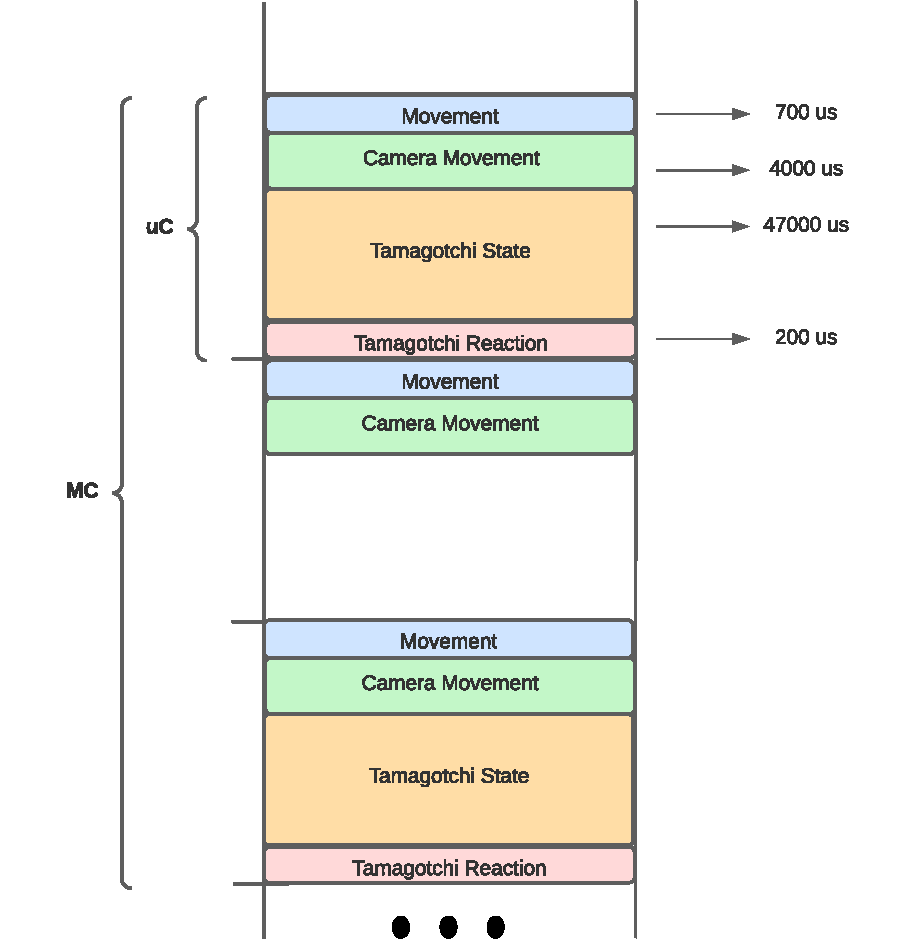
\includegraphics[width=\linewidth]{img/schedule.pdf}
    \caption{Static Schedule}
    \label{fig:schedule}
\end{figure}


\section{Implementation Details}

\subsection{Shared Resources}

The different tasks use the files as a means of communication. The server uses Python Pickle \footnote{\url{https://docs.python.org/3/library/pickle.html}} to dump data on the images being captured and movement commands being received. The movement tasks access the command files to execute them and the tamagotchi state task accesses the latest camera footage to evaluate the colours being presented. The tamagotchi state task also saves the state of the mascot in a file for the tamagotchi reaction task to access.


\subsection{Server}

As mentioned before, due to complications with our scheduling algorithm, in order to have our program properly function, the server had to be run outside the scope of the scheduler. 

The server is responsible for:

\begin{enumerate}
    \item Acquire data from the camera
    \item Stream the camera footage and save the latest frames in the file system
    \item Serve the mascot's requests via HTTP
    \item Allow for HTTP requests for vehicle motion and camera motion commands
    \item Record the vehicle and camera motion commands in a file
\end{enumerate}

The web page provided by this server allows the user to see what the robot sees, as well as issue commands for the movement of the robot and the camera and obtain information on the colour desired by the mascot.

\subsection{Tamagotchi Tasks}

The \textit{tamagotchi\_state} task updates the mood of the mascot. This task implements a state machine and the state is saved in the file system, not only for persistence but also to be accessed by other tasks. When the state is changed, a timestamp is created. There is a deadline for request execution and an idle time. When the idle time passes, the tamagotchi requests a new colour, randomly from the colour list. During the request deadline, this task reads the last image recorded by the camera from a file and decides whether it has the dominant colour requested or not. Depending on the outcome of the request, the tamagotchi is either happy or sad for a certain time, then switching to the mentioned idle state that serves as a cool-down before the next request.

To detect the dominant colour of a given frame, the image is resized to one pixel and we analyse its colour. The difference between colours is calculated using a formula \cite{b3} aimed to weight the RGB components to better fit human perception:

\begin{equation}
    \begin{aligned}
        \left\{ 
            \begin{array}{cl} 
                \sqrt{2*\Delta R^2 + 4*\Delta G^2 + 3*\Delta B^2} & , \frac{R1 + R2}{2} < 128 \\ 
                \sqrt{3*\Delta R^2 + 4*\Delta G^2 + 2*\Delta B^2} & , \ otherwise 
            \end{array} 
        \right.
        \label{windoweq2}
    \end{aligned}
\end{equation}

The \textit{tamagotchi\_reaction} task is responsible for using the buzzer to give some feedback about the outcome of a tamagotchi's request. This task reads the tamagotchi's state file and only acts if the mascot is on the \textit{happy} or \textit{sad} state. Depending on the state, the buzzer pattern is different: 

\begin{itemize}
    \item two beeps if the user finds the colour in time
    \item one long beep if the user fails to complete the task
\end{itemize}

\subsection{Movement Tasks}

The \textit{movement} task is responsible for coordinating the motion of the robot. It initially polls the infrared sensors for proximity of obstacles, commanding the robot to stop accordingly. It then reads the commands given by the user from a file. If the movement requested corresponds to the forward motion, it will only execute it if the information from the sensors does not indicate the presence of an obstacle. All the other commands are free to be executed, so that the robot can escape from dead ends.

The \textit{camera\_movement} task is responsible for coordinating the motion of the camera. It reads the commands given by the user from the same file as the movement task and executes them accordingly. It will adjust the PWM pulse sent to the camera servo motors (horizontal and vertical movement), according to the desired direction.

\section{Results}

The robot is able to comply with all the requirements. At maximum velocity, the robot is able to stop about $2cm$ away from an obstacle. The user experience is smooth and the response times of the system are satisfactory and meet the requirements. 

The website used for the control of the robot is depicted in Fig \ref{fig:website}.

We recorded a video \footnote{\url{https://youtu.be/Gruj3MmPWX4}} demonstrating the final result.

\begin{figure}
    \centering
    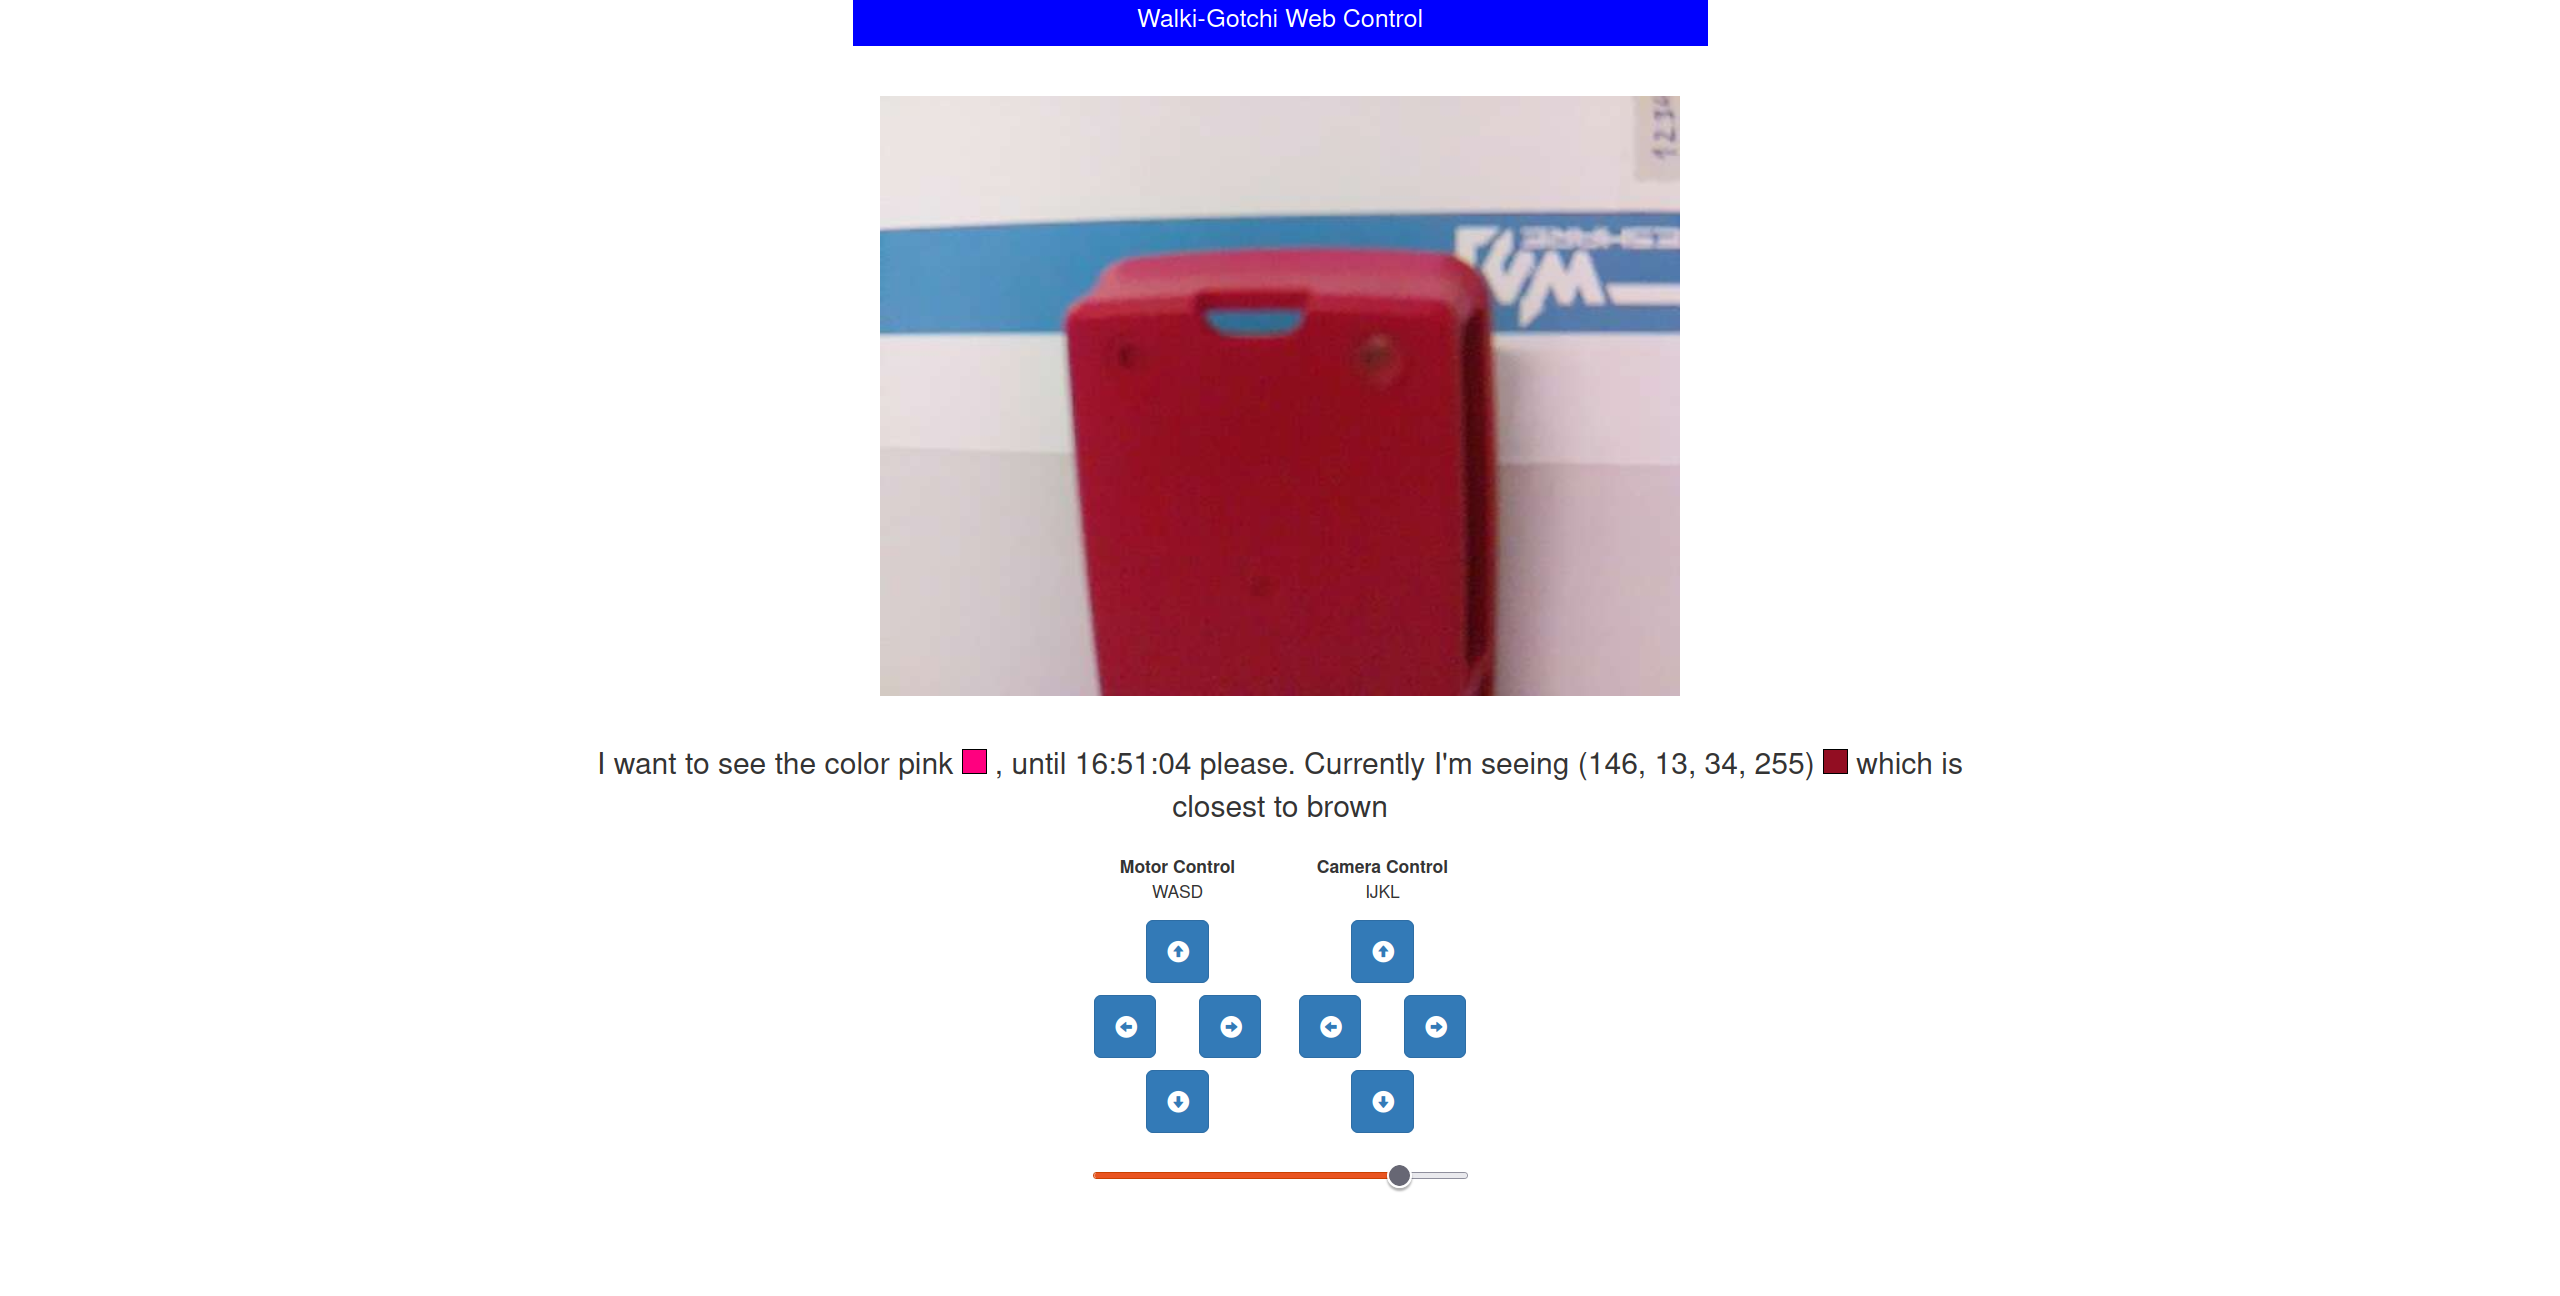
\includegraphics[width=\linewidth]{img/website.png}
    \caption{Website}
    \label{fig:website}
\end{figure}


\section{Conclusion}

The development of the project was riddled with difficulties inherent to the nature of the programming of embedded real-time systems. Despite the challenges, we are fairly content with the resulting system, believing it to be quite an intriguing and interesting idea successfully put into action. Moreover, the difficulties that arose along the development of the project represented many more learning opportunities that were well utilised, giving us better insight on what programming real-time systems really is. In sum, given the objectives of this course and of the proposed project, we consider our work a success.

\section{Contributions}

\begin{itemize}
    \item Marcelo Couto - 33\% 
    \item Lucas Santos - 33\%
    \item José Ferreira - 33\%
\end{itemize}


\begin{thebibliography}{00}
\bibitem{b1} Lehoczky, J., Sha, L., \& Ding, Y. (1989, December). The rate monotonic scheduling algorithm: Exact characterization and average case behavior. In RTSS (Vol. 89, pp. 166-171).
\bibitem{b2} Liu, C. L., \& Layland, J. W. (1973). Scheduling algorithms for multiprogramming in a hard-real-time environment. Journal of the ACM (JACM), 20(1), 46-61.
\bibitem{b3} Colour difference formula, close to human perception, retrieved from \url{https://en.wikipedia.org/wiki/Color\_difference}.

\end{thebibliography}

\newpage
\appendix

\begin{figure}[h]
    \centering
    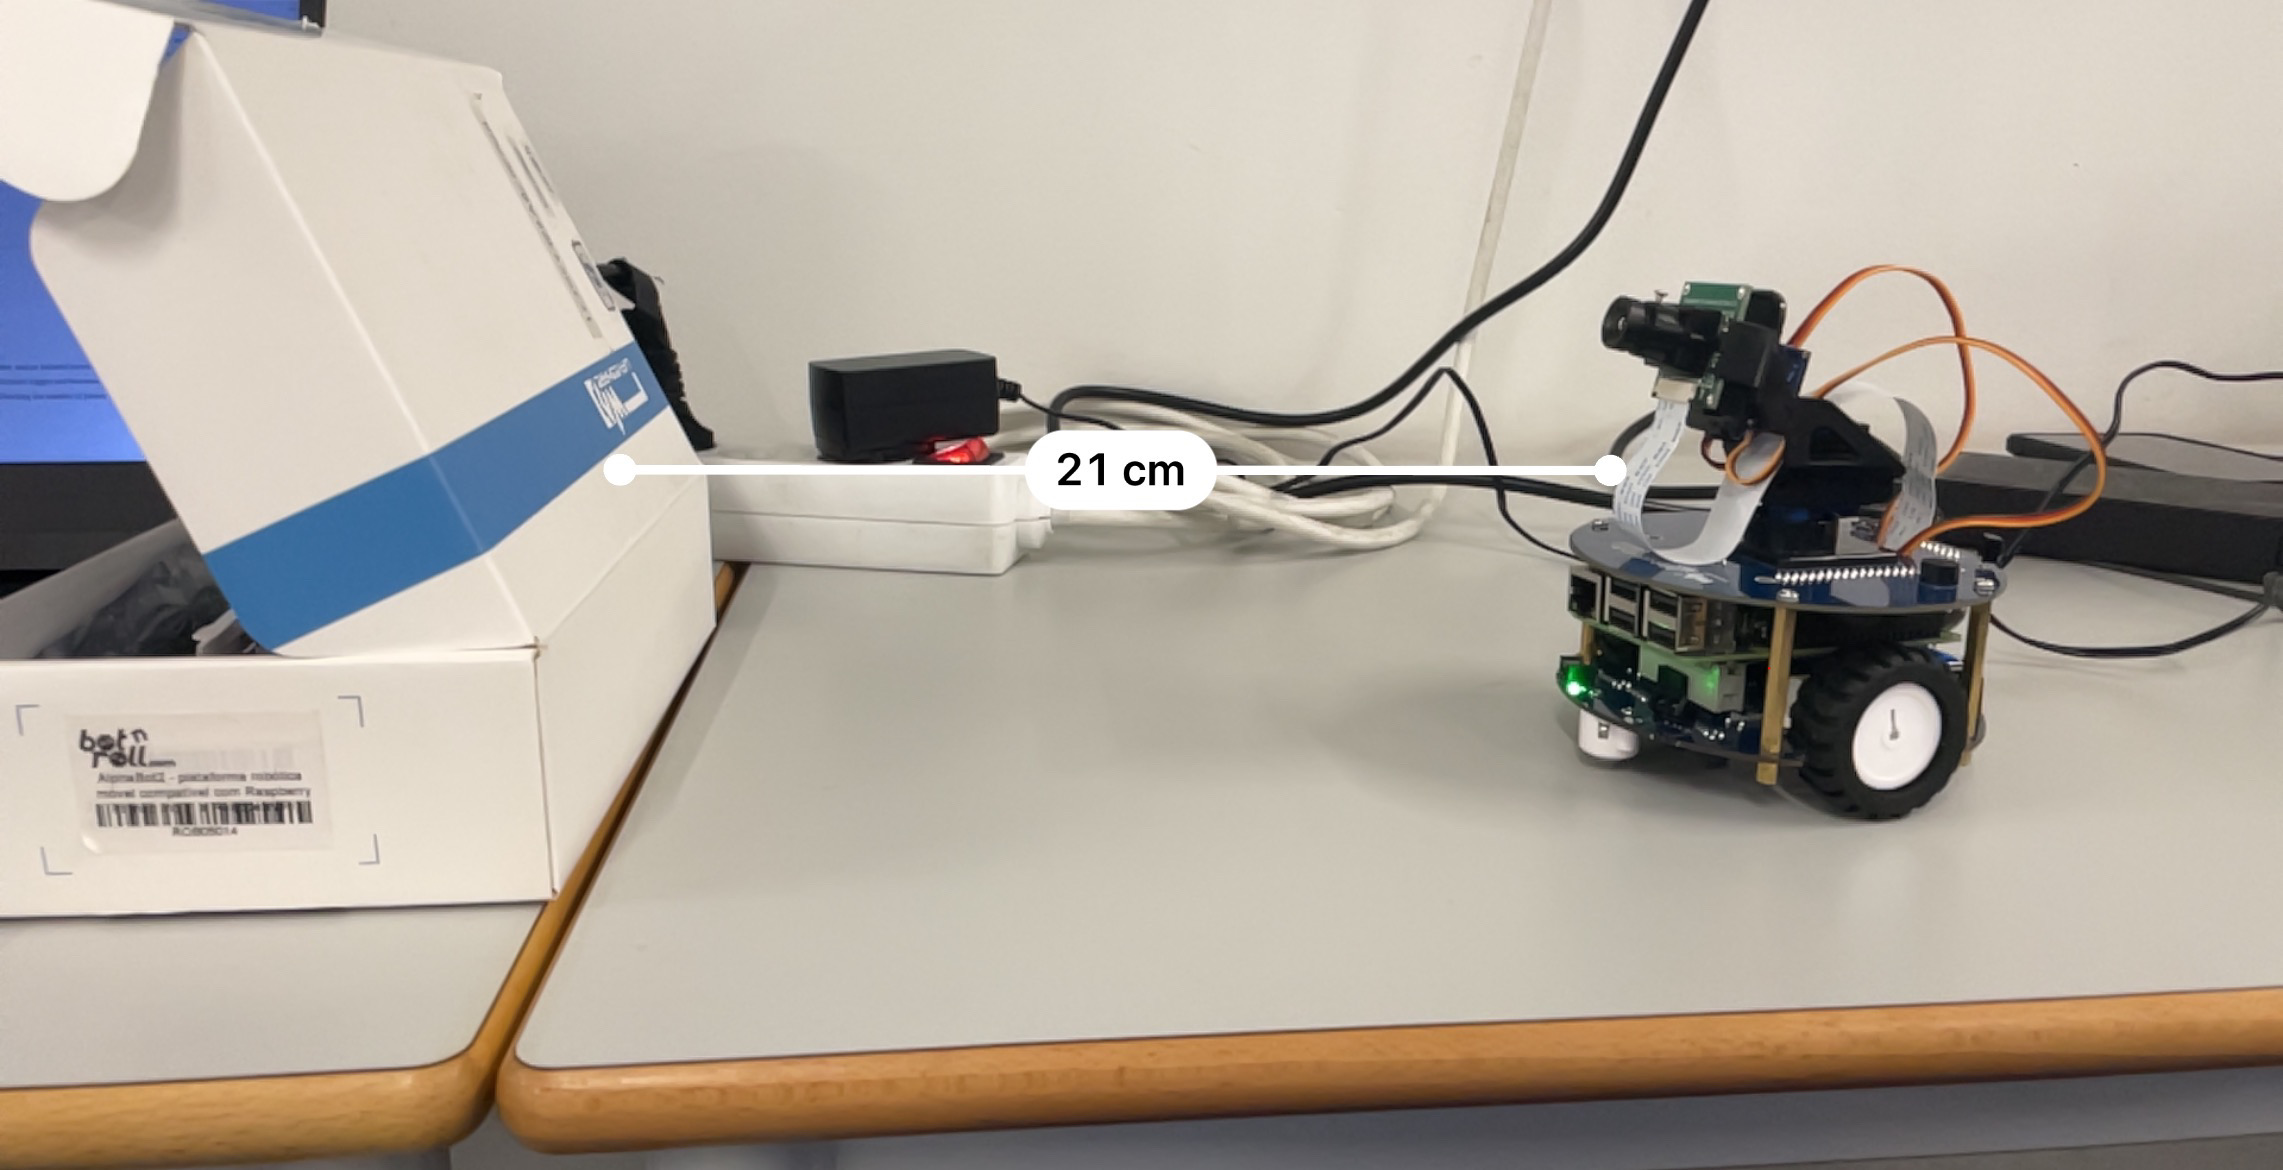
\includegraphics[width=\linewidth]{img/distance.jpg}
    \caption{Distance for sensor activation}
    \label{fig:distance}
\end{figure}

\begin{figure}[h]
    \centering
    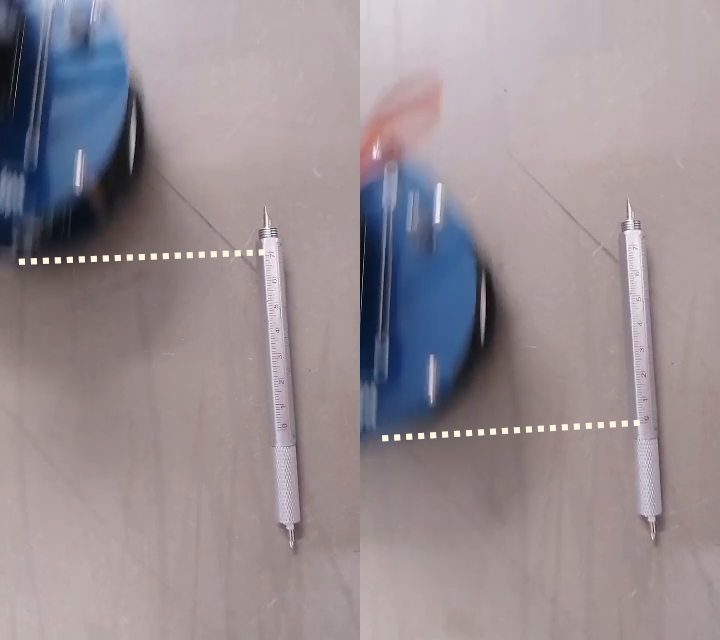
\includegraphics[width=\linewidth]{img/frames.png}
    \caption{Analysis of the robot's velocity}
    \label{fig:frames}
\end{figure}


\end{document}
